%***********************************************************
\subsection{MCMC Convergence}\label{sub:bc_mcmc_convergence}
%***********************************************************

\begin{figure}[!bth]
    \centering
    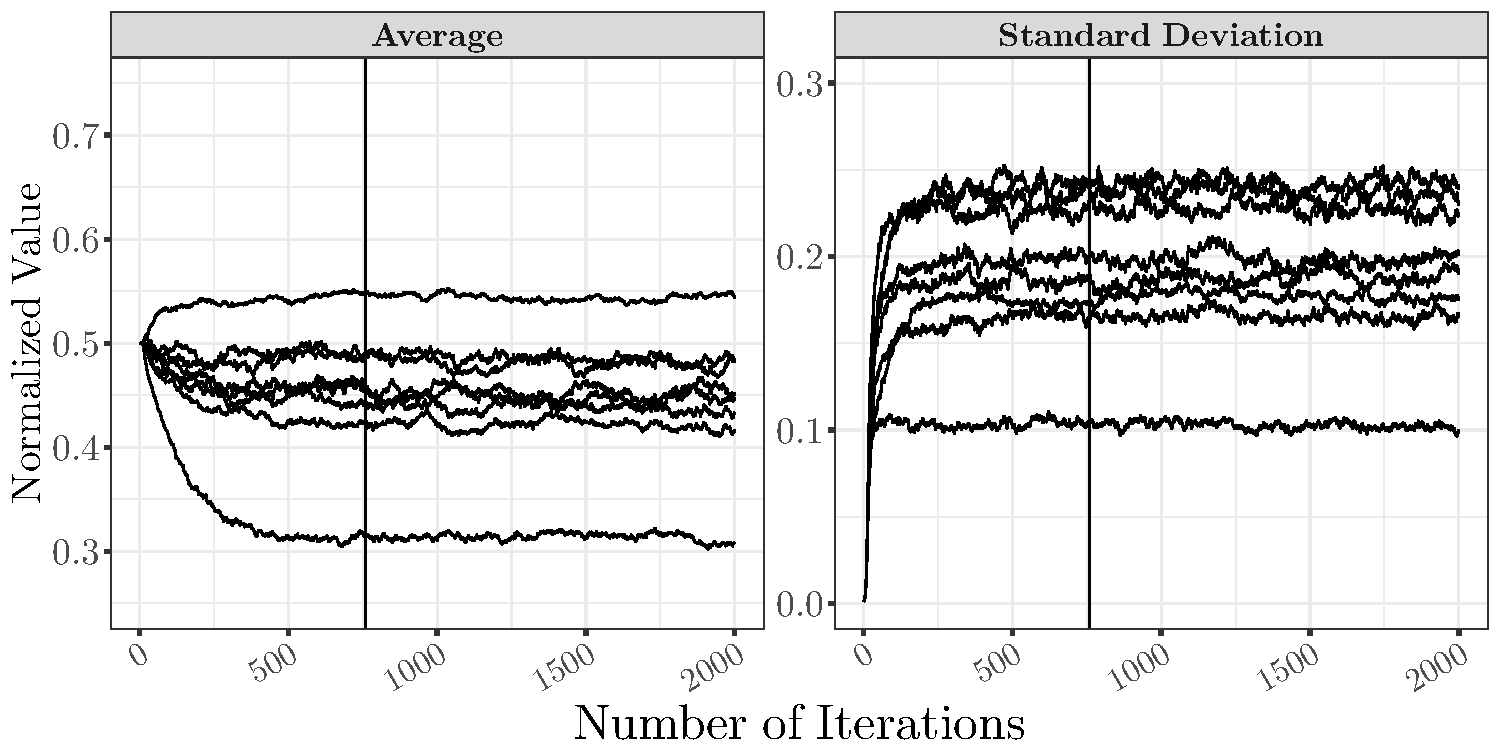
\includegraphics[width=1.0\textwidth]{../figures/chapter5/figures/plotEnsStatMCMC}
    \caption[Ensemble average and standard deviation as function of the number of iterations for calibration with model bias term.]{Ensemble average and standard deviation as function of the number of iterations for calibration with model bias term. Vertical lines indicate the iterations for burn-in (i.e., approximately $10$ times the autocorrelation time).}
    \label{fig:ch5_plot_ens_stat_mcmc}
\end{figure}

\begin{table}[h]
	\myfloatalign
	\caption[Estimated autocorrelation times for the $8$ model parameters with respect to the ensemble running average and standard deviation.]{Estimated autocorrelation times for the $8$ model parameters with respect to the ensemble running average and standard deviation. Bold term indicate the largest autocorrelation time used to determine the burn-in iterations.}
	\label{tab:ch5_ens_stat_mcmc}
	\begin{tabularx}{1.05\textwidth}{rlccccc} \toprule
		\multirow{2}{*}{No.}			&\multirow{2}{*}{Parameter}		&\multicolumn{2}{c}{Average}	&\phantom{a}&\multicolumn{2}{c}{Standard Deviation}\\
																															\cmidrule{3-4}	\cmidrule{6-7}
															&															& $\tau_{\text{pre-burn-in}}$ 		& $\tau_{\text{post-burn-in}}$	&& $\tau_{\text{pre-burn-in}}$ & $\tau_{\text{post-burn-in}}$ \\ \midrule
		1	&	\texttt{gridHT}				& \footnotesize{$7$}  				& \footnotesize{$22.43 \, [K] $} 	&& \footnotesize{$7$}  					& \footnotesize{$22.43 \, [K] $}\\
		2	&	\texttt{iafbWHT} 			& \footnotesize{$10$} 				& \footnotesize{$77.95 \, [Pa]$} 	&& \footnotesize{$7$}  					& \footnotesize{$22.43 \, [K] $}\\
		3	&	\texttt{dffbWHT} 			& \footnotesize{$5$}  				& \footnotesize{$ 0.27 \, [kg]$} 	&& \footnotesize{$7$}  					& \footnotesize{$22.43 \, [K] $}\\
		4	&	\texttt{dffVIHT}			& \footnotesize{$5$}  				& \footnotesize{$ 0.27 \, [kg]$} 	&& \footnotesize{$7$}  					& \footnotesize{$22.43 \, [K] $}\\
		5	&	\texttt{iafbIntDr} 		& \footnotesize{$5$}  				& \footnotesize{$ 0.27 \, [kg]$} 	&& \footnotesize{$7$}  					& \footnotesize{$22.43 \, [K] $}\\
		6	&	\texttt{dffbIntDr} 		& \footnotesize{$5$}  				& \footnotesize{$ 0.27 \, [kg]$} 	&& \footnotesize{$7$}  					& \footnotesize{$22.43 \, [K] $}\\
		7	&	\texttt{dffbWDr}			& \footnotesize{$5$}  				& \footnotesize{$ 0.27 \, [kg]$} 	&& \footnotesize{$7$}  					& \footnotesize{$22.43 \, [K] $}\\
		8	&	\texttt{tQuench} 			& \footnotesize{$5$}  				& \footnotesize{$ 0.27 \, [kg]$} 	&& \footnotesize{$7$}  					& \footnotesize{$22.43 \, [K] $}\\
		\bottomrule
	\end{tabularx}
\end{table}
